\documentclass[11pt,a4paper]{article}
\usepackage[T1]{fontenc}
\usepackage[utf8]{inputenc}

\usepackage[margin=2.3cm]{geometry}
\usepackage{mathptmx}
\usepackage[expansion=false]{microtype}
\usepackage{graphicx}
\usepackage{booktabs}
\usepackage{amsmath}
\usepackage{xcolor}
\usepackage{pgfplots}
\pgfplotsset{compat=1.17}
\usepackage[hidelinks]{hyperref}
\usepackage{caption}
\captionsetup{font=small,labelfont=bf}
\definecolor{ochre}{HTML}{B7802F}

\title{\textbf{Shared Sky}\\[4pt]\large The night sky of any place and moment laid onto the Earth,\\ with every tracked object in orbit passing through it}
\author{Sofia Gallego\\[2pt]
\small CosmoVentures, Paris, France\\
\small \href{https://sofiagallego.com}{sofiagallego.com}}
\date{\small YOHAKU hackathon (Space4Innovation), 25--27 September 2026\\
Challenge 1: \emph{Caring for Sky Country} \quad·\quad Challenge 2: \emph{Seven Generations in Orbit}}

\begin{document}
\maketitle

\begin{abstract}
\noindent Shared Sky is an open-source web application that shows the night sky above any place and moment laid one-to-one onto the land below it, together with constellations from fifteen sky cultures and all 31{,}225 objects in the public orbital catalogue. The mapping is the one used in celestial navigation: every star sits over the point on Earth where it is overhead, so one degree of sky equals 111.2~km of ground. Seen this way, satellites and debris stop being an abstract number and become things that cross one's own sky and one's own constellations. A second part, \emph{Seven generations in orbit}, estimates how long each object will stay in orbit, shows that about 11{,}900 of them will likely still be there in 175 years, and ranks which pieces could be taken care of first according to values that the user sets openly. The aim is awareness rather than prescription: the sky is shared by everyone beneath it, and most of the people under it never chose what now crosses it.

\smallskip
\noindent\textbf{Live:} \href{https://sofiagallego.com/shared-sky/}{sofiagallego.com/shared-sky} \quad \textbf{Code:} \href{https://github.com/nefinia/shared-sky}{github.com/nefinia/shared-sky}
\end{abstract}

\section{Motivation}
The sky has always been shared. Many cultures read the same stars as different figures, stories and calendars: the Kamilaroi and Euahlayi see an Emu in the dark lanes of the Milky Way, the Boorong a Jacky lizard, \emph{Unurgunite}, near Sirius. Over the last few years that shared sky has changed faster than ever. More than half of the objects tracked in orbit today were launched after 2020 (Fig.~\ref{fig:years}). Yet debris is usually shown as a cloud of dots around a globe, far from anyone's own night.

Shared Sky starts from the other end: from a person standing at a place, under their own sky and, where possible, their own constellations. It asks what crosses that sky, who put it there, and how long it will stay.

\begin{figure}[t]
\centering
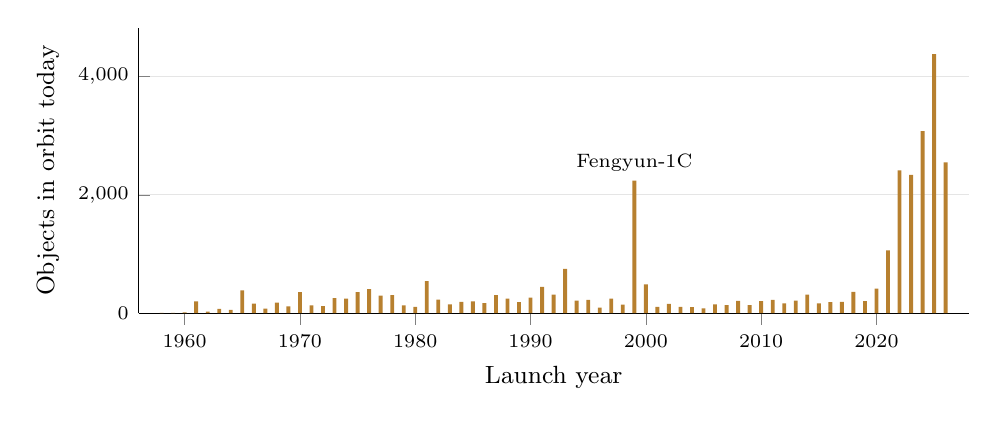
\begin{tikzpicture}
\begin{axis}[width=\linewidth,height=5.2cm,ybar,bar width=1.4pt,xmin=1956,xmax=2028,ymin=0,
  xlabel={Launch year},ylabel={Objects in orbit today},ylabel style={font=\small},xlabel style={font=\small},
  tick label style={font=\scriptsize},axis lines*=left,ymajorgrids,grid style={gray!20},
  xtick={1960,1970,1980,1990,2000,2010,2020},x tick label style={/pgf/number format/1000 sep=}]
\addplot[fill=ochre,draw=none] coordinates {(1958,3) (1959,5) (1960,11) (1961,199) (1962,24) (1963,70) (1964,54) (1965,384) (1966,159) (1967,77) (1968,179) (1969,114) (1970,354) (1971,132) (1972,117) (1973,255) (1974,244) (1975,357) (1976,404) (1977,295) (1978,305) (1979,133) (1980,107) (1981,543) (1982,227) (1983,146) (1984,189) (1985,199) (1986,170) (1987,303) (1988,246) (1989,187) (1990,262) (1991,442) (1992,311) (1993,747) (1994,213) (1995,222) (1996,94) (1997,246) (1998,145) (1999,2240) (2000,485) (2001,104) (2002,155) (2003,107) (2004,101) (2005,80) (2006,148) (2007,134) (2008,206) (2009,136) (2010,204) (2011,223) (2012,163) (2013,213) (2014,313) (2015,167) (2016,185) (2017,192) (2018,361) (2019,201) (2020,415) (2021,1060) (2022,2415) (2023,2338) (2024,3077) (2025,4378) (2026,2550)};
\node[font=\scriptsize,anchor=south] at (axis cs:1999,2240) {Fengyun-1C};
\end{axis}
\end{tikzpicture}
\caption{The 31{,}225 objects in the public catalogue (CelesTrak, 25 September 2026), by the launch year of the object they came from. Fragments inherit their parent's year: the 1999 peak is mostly the 1{,}969 tracked pieces of the Fengyun-1C satellite, destroyed in an anti-satellite test in 2007. 16{,}233 objects were launched in 2020 or later, 10{,}689 of them Starlink satellites.}
\label{fig:years}
\end{figure}

\section{The sky laid onto the land}
A star at zenith distance $z$ and azimuth $A$ is directly overhead at the point on Earth an arc $z$ away along bearing $A$: its \emph{geographic position}, the same idea navigators use. For a star of right ascension $\alpha$ and declination $\delta$ at Greenwich sidereal time $\theta_G$,
\begin{equation}
\phi_\star = \delta, \qquad \lambda_\star = \alpha - \theta_G .
\end{equation}
Drawing the Earth in orthographic projection centred on the observer then places land and sky on one picture, with a single scale: $1^\circ$ of sky $= 111.2$~km of ground. The observer's zenith sits on their spot and their horizon is a great circle $10{,}008$~km away, exactly half of the Earth. A constellation lies over the part of the world where it is overhead. The subsolar point is found the same way, which gives a real day and night terminator on the globe.

Objects in orbit are propagated with SGP4 from their two-line elements and can be drawn two ways: \emph{as seen in your sky}, lined up with the stars, or \emph{physically overhead}, over the ground they are flying above. Four views show the same scene: the sky on the land (the one-to-one map over real relief), standing there in 3D, one figure (a long exposure of every object crossing one constellation) and the whole sky.

\begin{figure}[t]
\centering
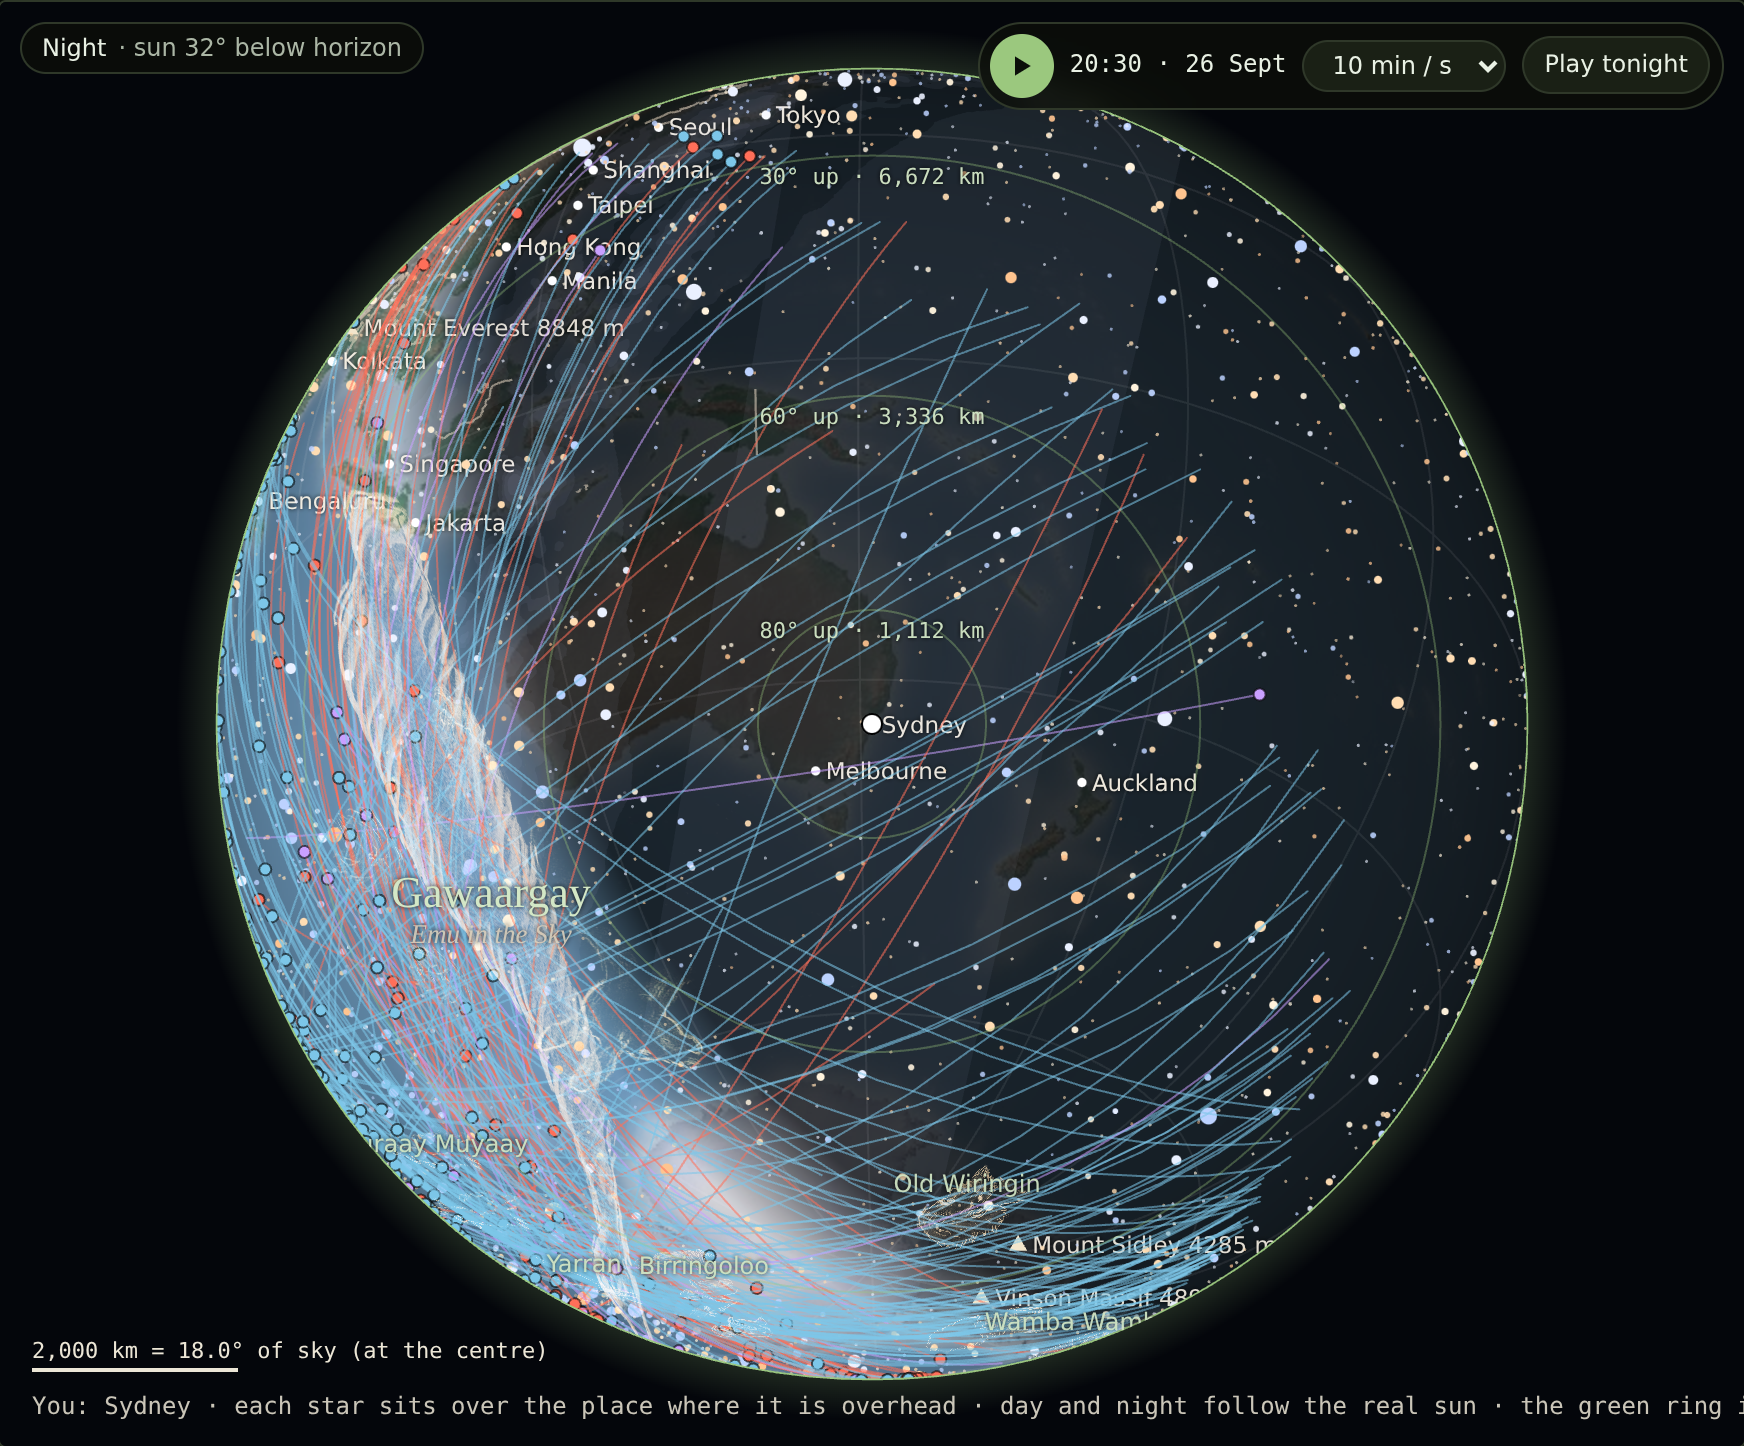
\includegraphics[width=.72\linewidth]{figures/sky-on-land.png}
\caption{\emph{Sky on the land} over Sydney (Gadigal Country) with the Kamilaroi/Euahlayi sky. Each star sits over the place where it is overhead; the green ring is the observer's horizon. Coloured paths are real objects over the next minutes: debris (red), rocket bodies (violet), satellites (blue).}
\label{fig:land}
\end{figure}

\section{Many skies, on their terms}
The fifteen sky cultures come from openly licensed Stellarium contributions, each credited in the application: among them Kamilaroi/Euahlayi, Boorong, Māori, Navajo, Blackfoot, Inuit, Tukano and Tupi-Guarani, alongside the Western constellations. They are listed together in one alphabetical list, and by default the page opens with the sky culture closest to the chosen place.

Many skies are missing, among them Mapuche, Lakota, Maya Kaqchikel, Shuar, Gadigal and Samburu. We found no open dataset for them, and they should be added only if those communities choose to, on their terms. The project follows the CARE principles for Indigenous data governance (Collective benefit, Authority to control, Responsibility, Ethics). Any request from a knowledge holder to correct, re-describe or remove a figure comes first.

\section{Seven generations in orbit}
Challenge~2 asks how we can decide which pieces of space debris humanity should take responsibility for first. The title recalls the seven-generations principle of the Haudenosaunee Confederacy: decisions should consider their effect seven generations ahead. With a generation of about 25 years, that is about 175 years.

\paragraph{How long each object stays.} From each orbit we compute the perigee and apogee heights and estimate a lifetime from a rule of thumb for decay time by height at average solar activity (about a year at 400~km, 25--30 years at 600~km, 150 years at 750~km, many centuries above 900~km). This is rough: real lifetimes vary several-fold with solar activity and each object's shape and mass. With it, about 11{,}900 of the 31{,}225 objects will likely still be in orbit seven generations from now.

\paragraph{Four values.} Each object gets four normalised factors:
\begin{itemize}\itemsep1pt
\item $T$, \emph{future generations}: its lifetime, counted up to the seven-generation horizon;
\item $C$, \emph{crowding}: how many tracked objects share its height band, per unit volume;
\item $M$, \emph{size}: a typical mass for its kind, raised to the power $0.75$, as the number of collision fragments grows with mass in NASA's standard breakup model;
\item $A$, \emph{shared skies}: the fraction of the Earth's surface its orbit passes over, $\sin i$ for inclination $i$.
\end{itemize}
The score is $S = T^{w_T}\,C^{w_C}\,M^{w_M}\,A^{w_A}$, where the weights $w$ are sliders the user moves. A weight of zero leaves that value out.

\paragraph{What it shows.} With equal weights, the first twenty are nineteen Soviet-era SL-16 upper stages (about 9~t each, launched 1987--2007, near 840~km) and one Chinese CZ-2C stage. Valuing only the long future brings objects launched from 1958 onwards to the top; valuing only crowding brings fragments near 460~km that will fall within a few years. The ranking is not an answer. It shows that \emph{first} depends on what we value, and makes those values visible so that people can discuss them together. Of the long-lived objects crossing the sky over Sydney, 34\% are registered to Russia or the former USSR, 28\% to the United States and 23\% to China: the people under a sky are rarely the ones who put anything in it.

\begin{figure}[t]
\centering
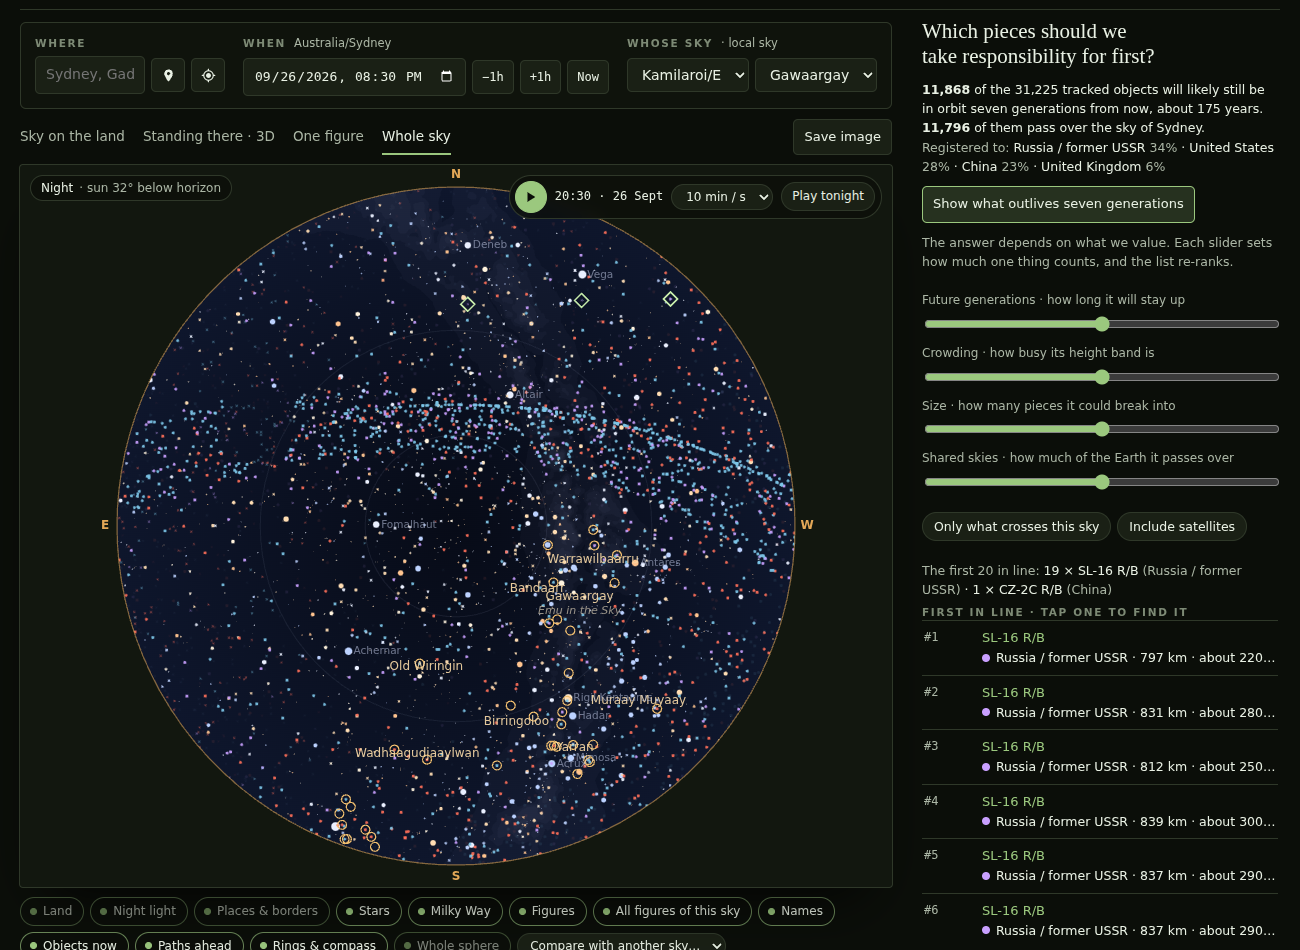
\includegraphics[width=\linewidth]{figures/seven-generations.png}
\caption{The whole sky over Sydney with the seven-generations view on. Objects that will come down on their own are dimmed; diamonds mark the first twenty in line under the current weights. Right: the headline figures, the four sliders and the ranked list.}
\label{fig:gen}
\end{figure}

\section{One figure, two skies}
Figure~\ref{fig:twoskies} shows Unurgunite, the Jacky lizard of the Boorong sky, over La Serena, Chile: on 17 March 1987 and on 27 September 2026. The stars have barely moved in a lifetime; what passes through them has. The 1987 view shows stars only, because orbits can be computed reliably only close to the date of the orbital data. It is not a record of an empty sky: at least 2{,}125 satellites and rocket stages launched by 1987 are still in orbit today.

\begin{figure}[t]
\centering
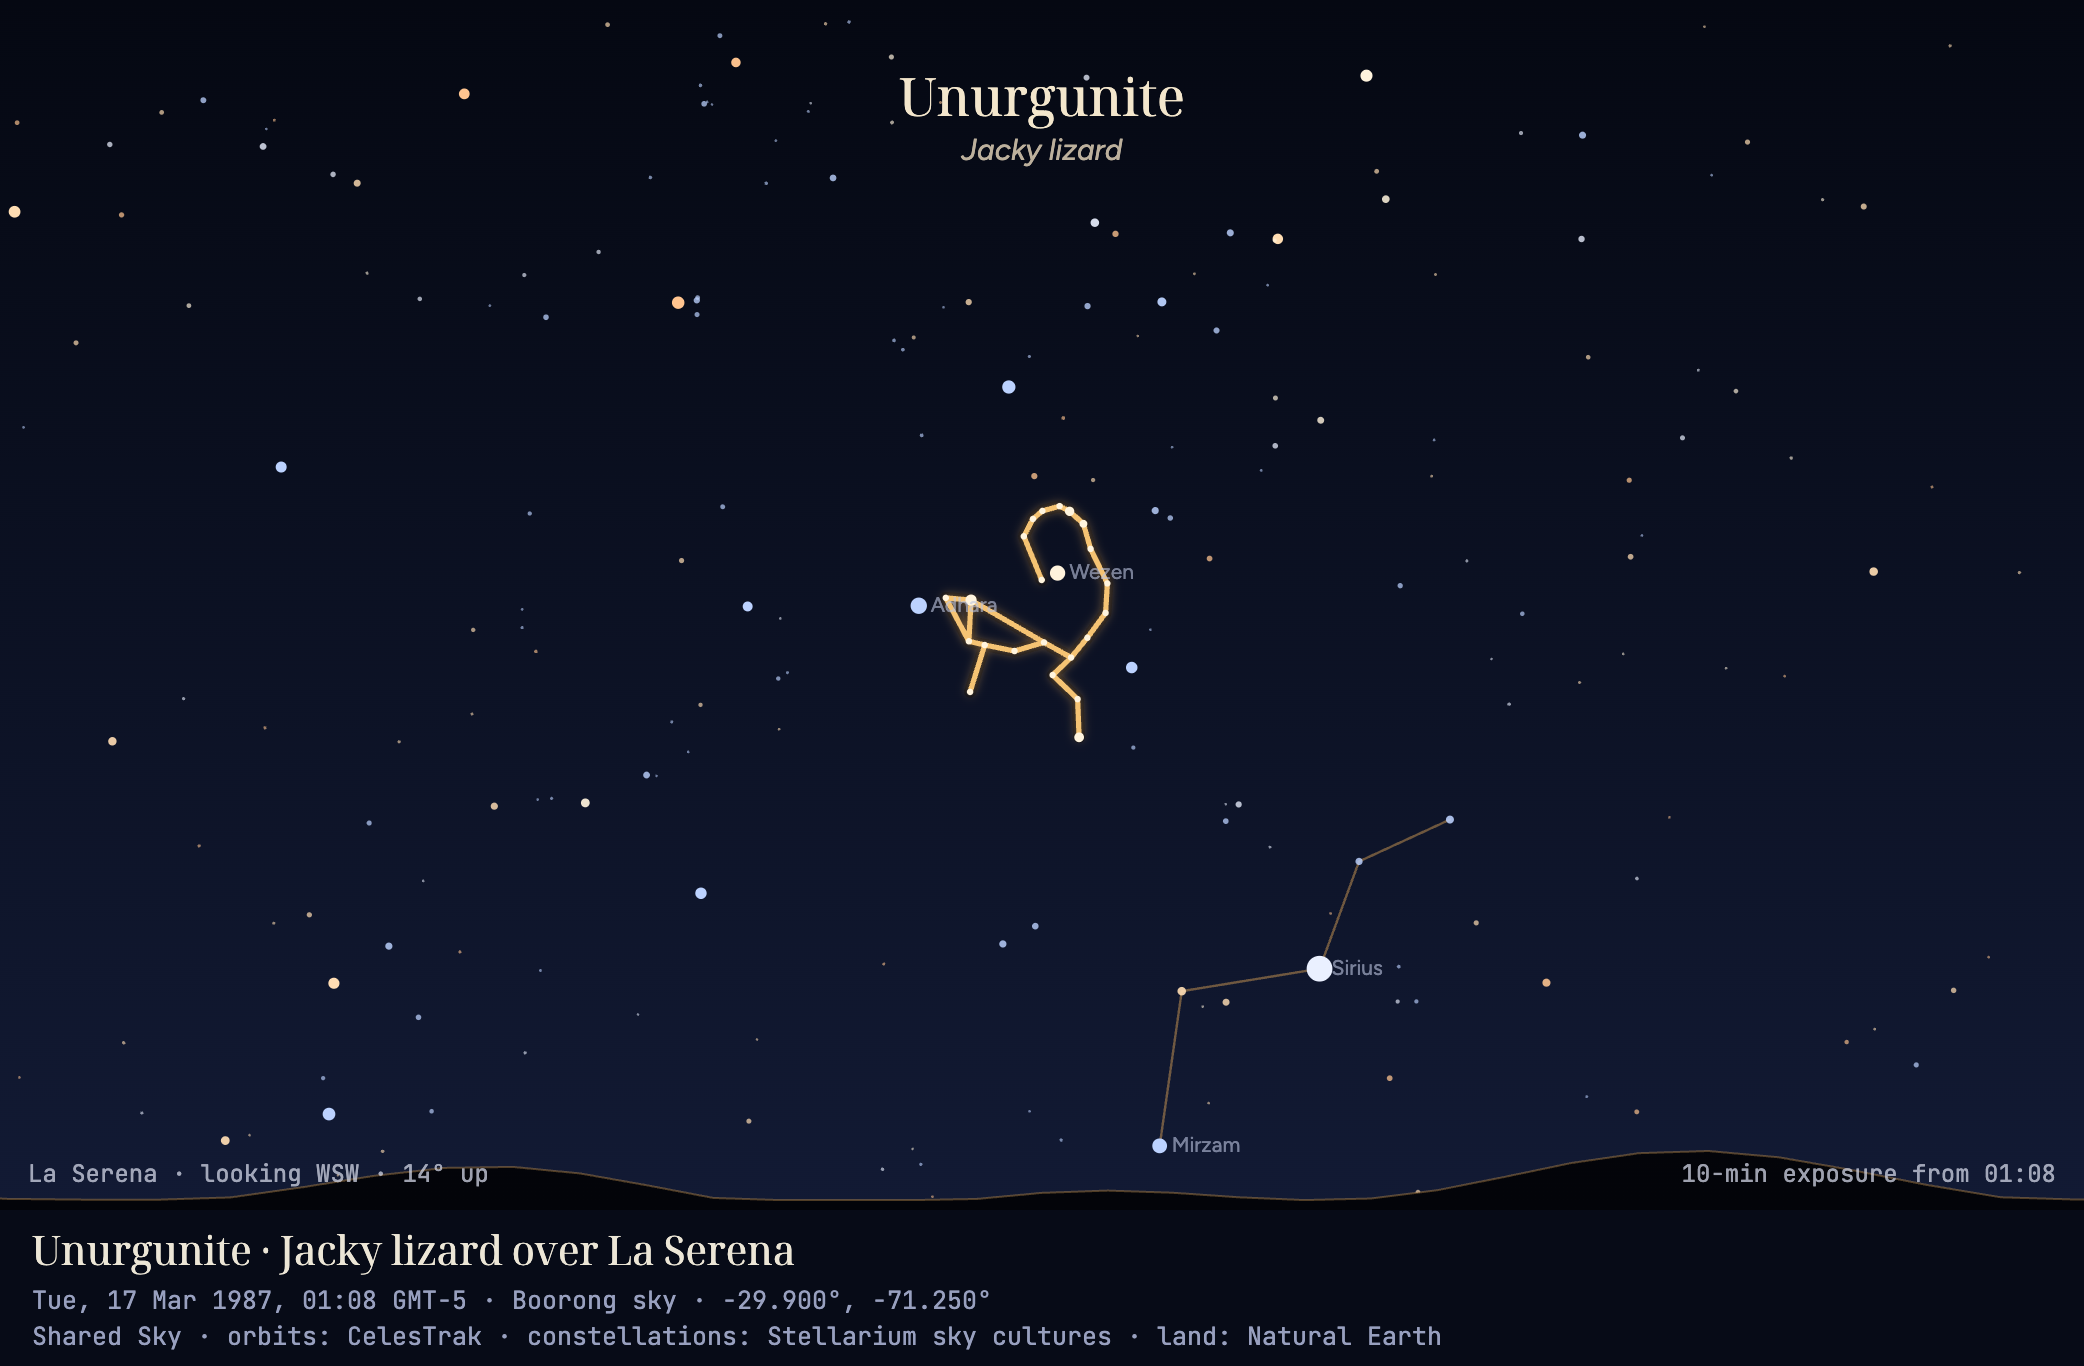
\includegraphics[width=.49\linewidth]{figures/unurgunite-1987.png}\hfill
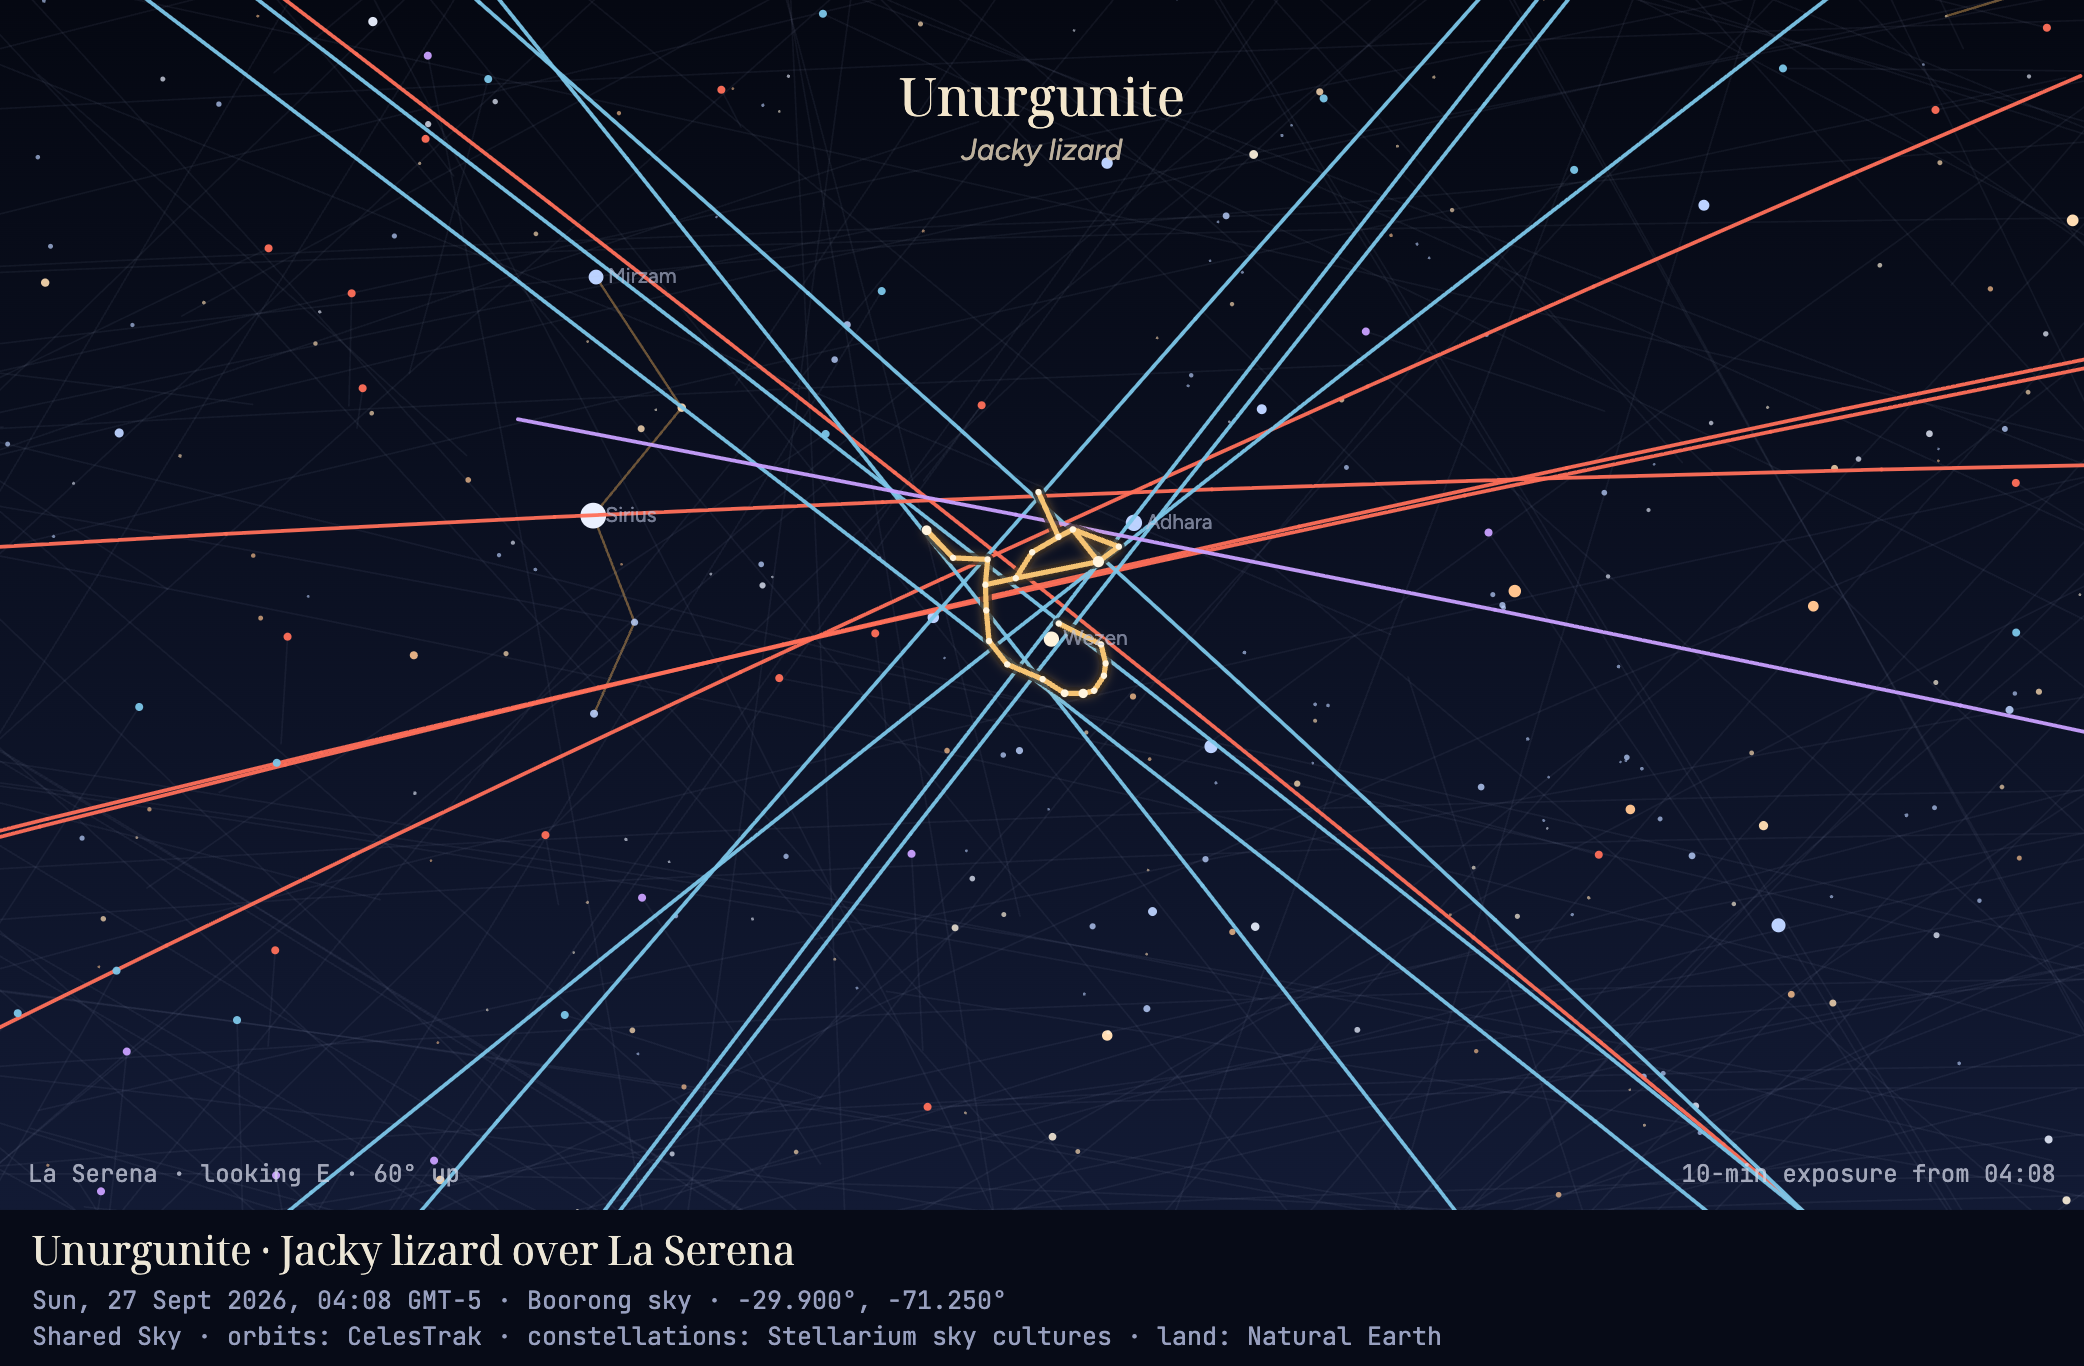
\includegraphics[width=.49\linewidth]{figures/unurgunite-2026.png}
\caption{Unurgunite over La Serena. Left: 17 March 1987 (stars only; see text). Right: 27 September 2026, a ten-minute exposure with every tracked object crossing the figure.}
\label{fig:twoskies}
\end{figure}

\section{Limits, stated plainly}
Debris positions come from one snapshot of the public catalogue and are reliable within about a week of it; a daily workflow keeps ``today'' covered. Only objects larger than about 10~cm are tracked; millions of smaller fragments are in no public catalogue. Lifetimes and masses are rough estimates. The 3D landscape is illustrative, while the one-to-one map uses real relief.

\section{What comes next}
\begin{itemize}\itemsep1pt
\item \textbf{Skies shared by the communities who hold them:} communities upload their own figures, names, stories and sound, choose who can see them, and can keep their data on their own server, so they can change or remove it at any time.
\item \textbf{Listening to the sky:} stars as notes on a pentatonic scale (brightness as loudness, colour as timbre, position as pitch), with passing objects adding their own sound.
\item \textbf{Deeper stewardship data:} lifetimes from measured drag and the solar cycle, uncertainty shown honestly, where re-entering objects come down and whose Country that is, and close approaches.
\item \textbf{Art tied to places:} artworks and stories attached to a place and a moment.
\end{itemize}

\section*{Responsible AI and credits}
\small
There is no AI inside Shared Sky: every number comes from open data and published formulas. AI (Claude, Anthropic) was used as a coding and writing assistant; the concept, direction and checks are the author's, and the author remains accountable for the tool and its limits.

Sky cultures: Stellarium sky-culture contributors and the knowledge holders behind them (each culture is credited in the application and in \texttt{CREDITS.md}). Orbits: CelesTrak public catalogue and SATCAT, propagated with satellite.js (SGP4). Land: Natural Earth. 3D: three.js. With thanks to the YOHAKU organisers and mentors. Code under the MIT licence; data keep their own licences.

\end{document}
